\documentclass{article}
\usepackage{graphicx}
\usepackage{amsmath}

\begin{document}

\begin{center}
\Large \textbf{Assembly Question}

\vspace{0.3cm}

Harshita N Kumar \\
COMETFWC052

\end{center}

\section*{Question}

Match the logic gates in Column A with their equivalents in Column B.

\begin{center}

\begin{tabular}{|c|c|}
\hline
\textbf{Column-A} & \textbf{Column-B} \\
\hline
1. AND GATE & P. XOR GATE \\
2. OR GATE & Q. XNOR GATE \\
3. NOT GATE & R. NAND GATE \\
 & S. NOR GATE \\
\hline
\end{tabular}

\end{center}

\begin{center}
\textbf{TABLE 11: Table-1}
\end{center}

\begin{itemize}
\item a) P-2, Q-4, R-1, S-3
\item b) P-4, Q-2, R-1, S-3
\item c) P-2, Q-4, R-3, S-1
\item d) P-4, Q-2, R-3, S-1
\end{itemize}

\section*{Solution}

Using logic identities:

$$
A \cdot B = (A \ NAND \ B)'
$$

$$
A + B = (A \ NOR \ B)'
$$

$$
A' = A \ XNOR \ 0
$$

Thus the correct matching is

$$
P-2,\ Q-4,\ R-1,\ S-3
$$

Hence the correct option is

\begin{center}
\textbf{a) P-2, Q-4, R-1, S-3}
\end{center}

\section*{Graph Output}

\begin{center}
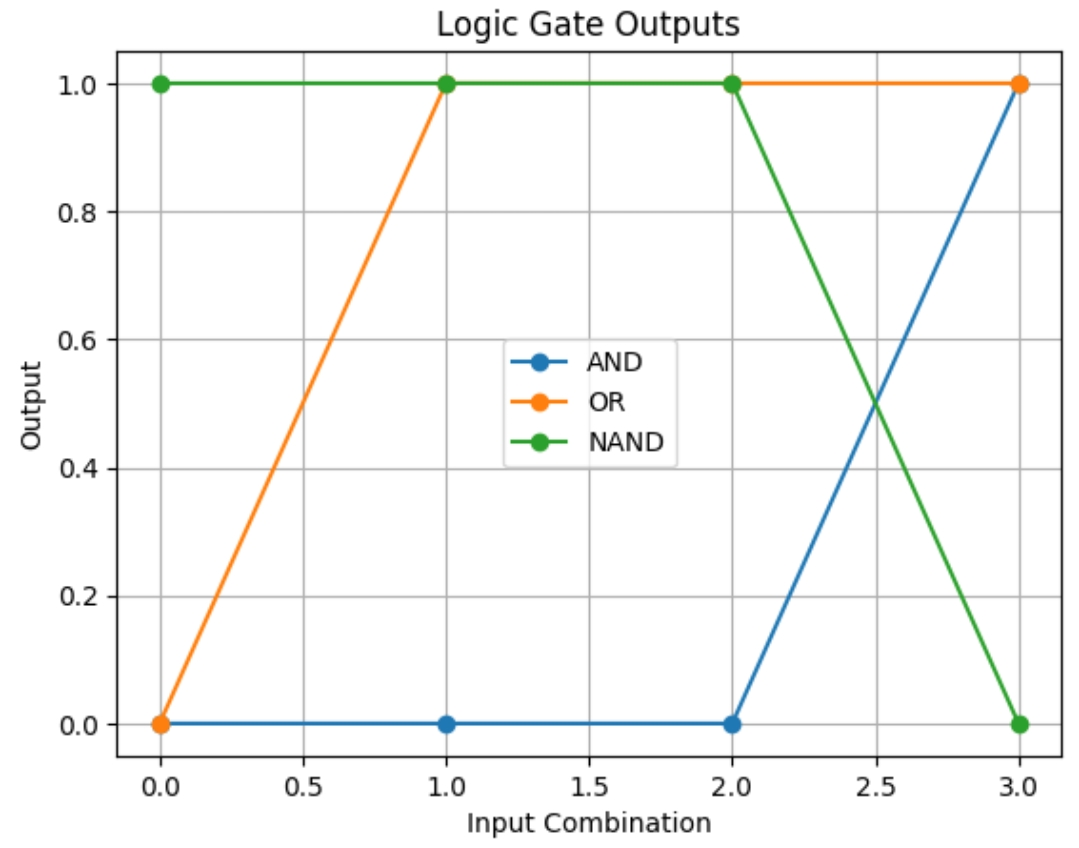
\includegraphics[width=12cm]{graph.jpg}
\end{center}

\end{document}
